\chapter{Method}
\label{chap:method}

We start of at the same spot we left of after the thesis. Before we go on to explain what's been done this semester, lets recap. 

We started off by just getting a drive with lots of \acrshort{das} data, and a script from \acrfull{asn} which set up us perfectly. We chose to rewrite python code to a language similar to that of MAtlab and Python. We landed on Julia, and with its broad ecosytstem it has support for all kinds of development we'd ever need. \\

We first wrote a 1:1 copy of the script, and then parallellized parts of the code until we had a version that could handle large amounts of data in parallel. We also wrote methods for being able to run a window over and \\ 




\section{Overview}

The \acrshort{api} that's being created is called \texttt{Judas} (Julia and DAS) and is split in 3 modules as well as a seperate Utils file as shown in \ref{fig:ccuda}

\begin{figure}[h]
    \centering
    \includegraphics{figures/overview.png}
    \caption{Overview over our package Judas}
    \label{fig:judasoverview}
\end{figure}

% Data
\section{Data}

For this project, we will be working with data recorded from BANE-NOR, where a train is travelling between Trondheim and Storen the 31st of august 2021. Data is split between 5000 sensor channels, lasting us a day.
The data is recorded in \acrshort{hdf5} files, with each file containing 20000 samples for 10 seconds, giving us a sample rate of $2000Hz$. The


\begin{table}[h]
\centering
\begin{tabular}{|r|r|r|r|r|}
\hline
\textbf{1}                & \textbf{2}               & \multicolumn{1}{c|}{\textbf{...}} & \textbf{n-1}             & \textbf{n}               \\ \hline
1f-3                      & 2.3f-5                   & 4f-4                              & 3.4f-6                   & 3f-1                     \\ \hline
3f-1                      & 3f-1                     & 3f-1                              & 3f-1                     & 3f-1                     \\ \hline
\multicolumn{1}{|c|}{...} & \multicolumn{1}{c|}{...} & \multicolumn{1}{c|}{...}          & \multicolumn{1}{c|}{...} & \multicolumn{1}{c|}{...} \\ \hline
4f-2                      & 3f-1                     & 3f-1                              & 3f-1                     & 3f-1                     \\ \hline
\end{tabular}
\caption{Table explaining how the table looks like}
\label{fig:datatable}
\end{table}



TODO: Figure over dataflow  

\subsection{Pre processing}

After the data has been loaded \cite{projthesis}, it's still not ready for processing. 

The function \lstinline|process_DAS_data| takes in the signal data, perform a tukey \ref{dsp:tukey} window algorithm over it. We then run a bandpass filter algorithm with Butterworth over it to extract the and 

\begin{figure}
    \centering
    \lstinputlisting{code/procdasdata.jl}
    \caption{Process DAS data function}
    \label{fig:procdasdata}
\end{figure}


After applying a window function and a filter function to combat oscilleration, we're now ready to run an fft over this data. 


The 

\begin{figure}[h]
    \centering
    \includegraphics{figures/banenor_20210831.png}
    \caption{Heatmap of the processed train data during the 31st of august 2021 from Trondheim to Storen}
    \label{fig:trdstrdas}
\end{figure}

\subsection{Data preparation before } 

Now that the data has been successfully pre-processed, we still need to 



\subsubsection{Data augmentation}


% NETWORK ARCH
\section{Network Architecture}

The model consists of

\begin{itemize}
    \item Batch size 
    \item skdfj
    \item sdfk
\end{itemize}

\begin{table}[h]
    \centering
    \begin{tabular}{ l c r }
      \hline
      Layer (type) & Output shape & Param \# \\ \hline
      lstm\_1 (LSTM) & (None, 10, 256) & 1234678 \\ \hline
      lstm\_1 (LSTM) & (None, 10, 256) & 1234678 \\ \hline
      lstm\_1 (LSTM) & (None, 10, 256) & 1234678 \\ \hline
      lstm\_1 (LSTM) & (None, 10, 256) & 1234678 \\ \hline
      lstm\_1 (LSTM) & (None, 10, 256) & 1234678 \\ \hline
      Total params: & & \\
      Trainable params: & & \\ 
      Non-Trainable params: 0 & & \\ \hline
      
    \end{tabular}
    \caption{Parameters for our architecture}
    \label{tab:archparams}
\end{table}


\begin{figure}[h]
    \centering
    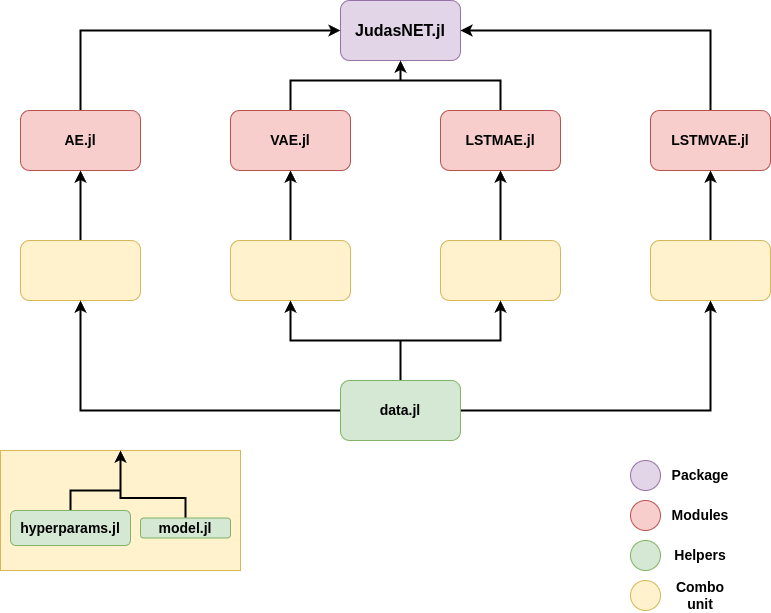
\includegraphics{figures/judasnet.png}
    \caption{JudasNET network architecture}
    \label{fig:judasnet}
\end{figure}


\subsection{Hyperparameters}

See \cite{app:hyperparams} for a detailed view on all the different hyperparameters used for this particular model



% DAS


The DAS folder has not changed much substantially. The main difference from before is how we now instead of writing matrix data to one large binary file, data is split into multiple files, and only read when needed.

Contrary to what was mentioned before, the output of the function \texttt{load\_DAS\_files} has actually changed. Previously, we stored a whole vector of the timestamps for each sample. Not only was this cistly, but actaully totally redundant. If the timestamp of the first row is known, the sampling rate $T$ and which row to look at, one can instead calculate the timestamp like this: 
\lstinline|start_time + MilliSecond(idx * T * 1000)|. This inplace calculation can be done multiple times effectively in Julia using the broadcast operator (.). This ensures that we don't lose essential information before running our data through through the autoencoder

\begin{figure}[h]
\centering
\begin{subfigure}{.5\textwidth}
  \centering
  \lstinputlisting{code/dasstructold.jl}
  \caption{Old DAS Struct}
  \label{fig:olddasstc}
\end{subfigure}%
\begin{subfigure}{.5\textwidth}
  \centering
  \lstinputlisting{code/dasstruct.jl}
  \caption{New Layout for DAS struct}
  \label{fig:newdasstc}
\end{subfigure}
\caption{Comparison between different versions of the DAS struct}
\label{fig:dasstccmp}
\end{figure}

\section{SignalProcessing.jl}

After data has been read and processed, it's ready to be processed by signal processing functions 

\section{AI.jl}

The main aspects of this code lies within the module \texttt{AI.jl}. 


\subsection{JudasNET}

\texttt{JudasNET} is the architecture of choice for interpreting data

\begin{figure}{h}
    \centering
    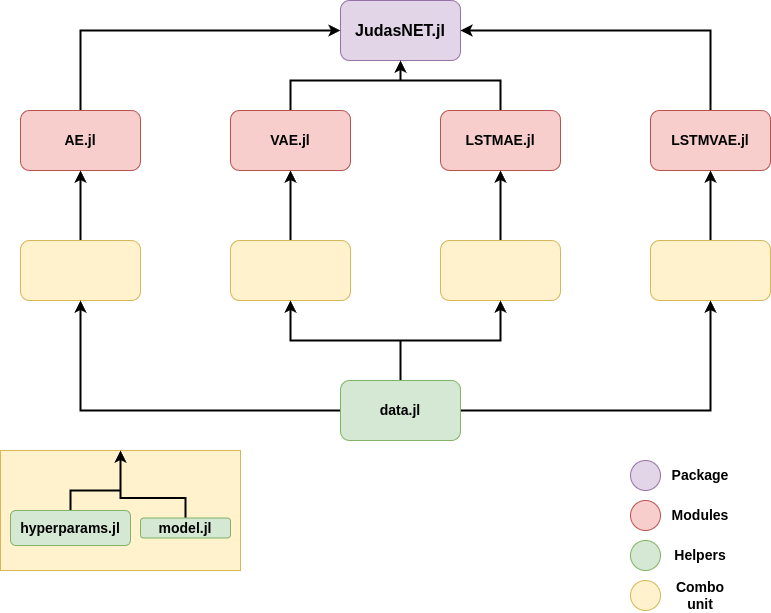
\includegraphics[scale=.6]{figures/judasnet.png}
    \caption{Flowchart over JudasNET}
    \label{fig:judasnet}
\end{figure}

\subsubsection{Modification to Flux.jl}

As mentioned previously, one of the main benefits with Julia packages is the ability to easily add new functionality to packages. When working with \texttt{Flux.jl}, this has certainly been useful. For our research, we had to write our own LSTM functors to be able to achieve a LSTM Autoencoder.  \\

The first of this functors is a regular LSTM, but with \texttt{relu} as the activation function for the different gates. Secondly, we rewrote the TimeDistributed layer \cite{keras} for Flux since there is no corresponding alternative as of the writeday of this paper. The final layer we had to recreate is what's known as a \texttt{RepeatVector} in Keras. When we have all of these together, we can finally put them together and write our model. 

\begin{figure}[h]
    \centering
    \lstinputlisting{code/judasnet.jl}
    \caption{JudasNET flux model}
    \label{fig:fluxjudasnet}
\end{figure}



We're using \acrfull{adam} as the choice of our optimizer

\begin{equation}
    \omega - \alpha \frac{v_{dw}}  {\sqrt{s_{dw}} + \epsilon}
\end{equation}